%!TEX TS-program = lualatex

%\documentclass[10pt]{article}


\documentclass[draft,jgrga]{agu_template/AGUTeX}

\usepackage[a4paper,left=2cm,top=2cm,right=3cm,bottom=2cm]{geometry}
\usepackage{amsmath}
\usepackage{amssymb}
\usepackage{amssymb}
\usepackage{graphicx}
\usepackage[makeroom]{cancel}
%\usepackage{enumitem}
%\usepackage{theorem}
%\usepackage{fancybox}
%\usepackage{subfigure,wrapfig}
\usepackage{bm}
%\usepackage{parskip}
%\usepackage{setspace}
%\usepackage{caption}
%\usepackage{fancyhdr}
%\usepackage[compact]{titlesec}
\usepackage{xargs}  % Use more than one optional parameter in a new command
\usepackage[prependcaption, textsize=tiny]{todonotes}

\graphicspath{FigurePDFs}

\definecolor{lmnotecol}{rgb}{1.0,0.4,0.0}
\newcommandx{\louis}[2][1=]{\todo[color=lmnotecol!50, #1]{LM:#2}}
\newcommandx{\comment}[2][1=]{\todo[color=blue!40,#1]{#2}}



%  Uncomment the following command to allow illustrations to print when using Draft:
\setkeys{Gin}{draft=false}


%% Layout (which might be better off in the individual document types)

%\setlength{\mathindent}{15mm}
%\setlength{\leftmargini}{0pt}
\setlength{\parindent}{0pt}
%

%\setstretch{1.3}

%\captionsetup{font={small,it},labelfont={bf,it}} 
%\titlespacing{\section}{0pt}{*0.5}{*2}
%\titlespacing{\subsection}{0pt}{*0.5}{*0.25}
%\titleformat{\subsubsection}[runin]{\normalfont \bfseries \itshape}{}{0pt}{} 
%\titlespacing{\section}{\parindent}{*2}{\wordsep}
%\setlength{\headheight}{14pt}
%\pagestyle{fancyplain}
%\pagenumbering{roman}

%\usepackage{url}
%\urlstyle{same}

% \usepackage{fontspec}  %% xelatex or luaLatex required
% \defaultfontfeatures{Scale=MatchLowercase,Mapping=tex-text}
% \setmainfont{Cambria}
% \setsansfont{Helvetica}
% \setmonofont{Courier New}

% \newcommand{\Tf}[2]{\textstyle\frac{#1}{#2}}

\setlength{\parskip}{1ex plus 0.5ex minus 0.2ex}


%----------------------------------------------------------------------------------------
%	RUNNING HEAD AND CORRESPONDING AUTHOR
%----------------------------------------------------------------------------------------

% Author names in capital letters:
\authorrunninghead{MORESI}

%------------------------------------------------

% Shorter version of title entered in capital letters:
\titlerunninghead{PARALLEL SURFACE PROCESSES}

%------------------------------------------------

% Corresponding author mailing address and e-mail address:
\authoraddr{Corresponding author: Louis Moresi, School of Earth Sciences, The University of Melbourne, Australia. (louis.moresi@unimelb.edu.au)}



\begin{document}

%----------------------------------------------------------------------------------------
%	TITLE
%----------------------------------------------------------------------------------------

\title{Surface Process Modelling approaches for highly parallel, decomposed domains}

%----------------------------------------------------------------------------------------
%	AUTHORS AND AFFILIATIONS
%----------------------------------------------------------------------------------------

% Use \author{\altaffilmark{}} and \altaffiltext{}

% \altaffilmark will produce footnote; matching \altaffiltext will appear at bottom of page.

\authors{Louis Moresi \altaffilmark{1}}

\altaffiltext{1}{School of Earth Sciences, The University of Melbourne, Australia}


%----------------------------------------------------------------------------------------
%	ABSTRACT
%----------------------------------------------------------------------------------------

% Do NOT include any \begin...\end commands within the body of the abstract.

\begin{abstract}

Lorem ipsum dolor sit amet, consectetur adipiscing elit. Sed vehicula metus sapien. Suspendisse pulvinar, felis ut hendrerit aliquet, dui nisi bibendum erat, fermentum mattis enim nibh id arcu. Vestibulum ultrices eros sed odio tincidunt bibendum. Pellentesque fermentum ante vel nulla commodo fermentum. Vestibulum in augue sit amet libero viverra accumsan eu at magna. Sed at ligula quis nibh pharetra facilisis non eu libero. Suspendisse non quam sit amet massa luctus interdum sit amet in purus. Integer id orci elit, vitae sollicitudin lectus.

\end{abstract}

\section{Introduction}

... Challenge to interpret the expression of geodynamic processes in the geological record. In particular we need to recognise the ephemeral nature of the surface signal of deep mantle flow and look for irreversible imprints which are stamped into the long-lived record. One of the most important of these is the erosion of topographic highs and associated 

Context - combining surface evolution models with large scale tectonic deformation models to understand the erosion / deposition / transport record and how it interacts with horizontal and vertical deformation. The latter makes it difficult to entirely decouple the two processes in a numerical sense.


We first produce a simplified erosion / deposition and transport model which captures just enough of the relevant processes to illustrate the essential characteristics of the problem. 

We then discuss the distinctive numerical difficulties which arise in developing a parallel approach to this problem within the context of a decomposed domain. 

We then show how a matrix-operator based formulation of the key processes leads to an efficient way to write and code the numerical surface process equations 

\section{Simple Erosion, Deposition and Transport Models}

We follow an approach outlined by ... ?? [which simple deposition model should we use ??]

The contributing processes to landscape evolution - local v. global ... 

\begin{equation}
  \frac{Dh}{Dt} =  \dot{h}_\textrm{local} 
  				 + \dot{h}_\textrm{incision} 
  				 + \dot{h}_\textrm{deposition}   
  				 + \dot{h}_\textrm{basement}
\end{equation}
$h$ is the surface height at each point, the $\dot{h}$ terms are time derivatives in the height, the derivative $D/Dt$ includes transport by horizontal motions of the basement, and $\dot{h}_\textrm{basement}$ accounts for vertical motion of the basement.

The local evolution rate represents small-scale, hill-slope dependent processes which can be represented as a non-linear diffusion equation. 
\begin{equation}
	\dot{h}(\bm{x})_\textrm{local} = \nabla \left[\kappa(h,\bm{x}) \nabla h(\bm{x}) \right]
\end{equation}  
$\kappa$ is a non-linear diffusion coefficient which can, for example, be used to enforce a 
critical hill slope value if it is a strongly increasing function of the local gradient.

The fluvial incision rate is more complicated in that it includes the effect of cumulative rainfall runoff across the landscape. This term depends on the available energy of rivers which in turn is related to both the discharge flux at any given point and the local stream-bed slope. In the so-called stream power form, the incision rate may be written as  

	\begin{equation}
		\dot{h}(\bm{x})_\textrm{incision} = 
				K(\bm{x}) q_r(\bm{x})^m \left| \nabla h(\bm{x}) \right|^n
	\end{equation}

Where $K$, $m$, $n$ are constants, $q_r$ is the runoff flux, and $\left| \nabla h \right|$ is the downhill bed slope.

	\begin{equation}
		q_r(\bm{x}) = \int\displaylimits_{\textrm{upstream}} \!\!\!\! {\cal R} (\xi) d \xi
	\end{equation}

\noindent
This integral computes the accumulated run off for all of the areas which lie upstream of the point $\bm{x}$. This term is strongly dependent on the geometry of the catchment and the connectivity of the network of tributaries above $\bm{x}$ and is generally not local, non-uniform in sampling the domain, and will change, potentially discontinuously, as the topography evolves.



%% [Does this belong here ?]

%\begin{equation}
%  \frac{Dh}{Dt} = \nabla \kappa(h) \nabla h +
%  				   K A^m \left| \nabla h \right|^n + 		   
%\end{equation}

%the first term on the right hand side represents hillslope evolution due to local slope-dependent processes as a non-linear diffusion equation ($\kappa$ is a non-linear diffusion coefficient). The second term on the right hand side is non-local and represents the influence of 

The counterpoint to the incision term is the rate of change of height due to deposition of sediment by the flow. This is controlled by the transport capacity of the water flowing past a point which, once saturated, prevents the further uptake of eroded material from the bed. 


Sklar \& Dietrich [] point out that the constant, $K$, in the stream power equation in fact bundles many physical processes that should depend upon emergent properties of the system including the sediment load carried by the streams. This implies a strong, additional non-linearity which we will not consider other than to point out that it is also an integral of an upstream quantity. 


FIGURE: Simple erosion model in terms of downstream flow

... 

Suppose we represent a landscape by heights recorded at discrete points which we can store on a triangulated (or other) mesh. Pathways taken by water flowing over the landscape can be constructed by connecting each point to whichever of its neighbours defines the steepest descent direction (which can be approximated by the lowest of the neighbours if the mesh is close to being regularly spaced). In concave regions of the landscape, these paths generally form a tree-like structure since points usually have a unique downhill neighbour, but several points may share the same downhill neighbour. A small segment taken from such a tree is illustrated in Figure \ref{fig:Tree} with the direction of the downhill flow indicated by the sense of the arrows.  

NETWORK STABLITY

[Something here about numerical efficiency of not recalculating network]

The erosion terms in the surface evolution equation [eq:...] which depend on the flow of water and sediment across the landscape naturally are localising and tend to focus further erosion in the existing channels. This effect stabilises the topology of the steepest-descent network over time. Where deposition occurs the reverse is true since channels tend to fill and local gradients reduce over time. Once gradients are low, deposition will quickly reconfigure the network and, in fact, it may not be particularly helpful to try to identify a single direction of flow from any given node [REF]


\begin{figure}[hbt]
  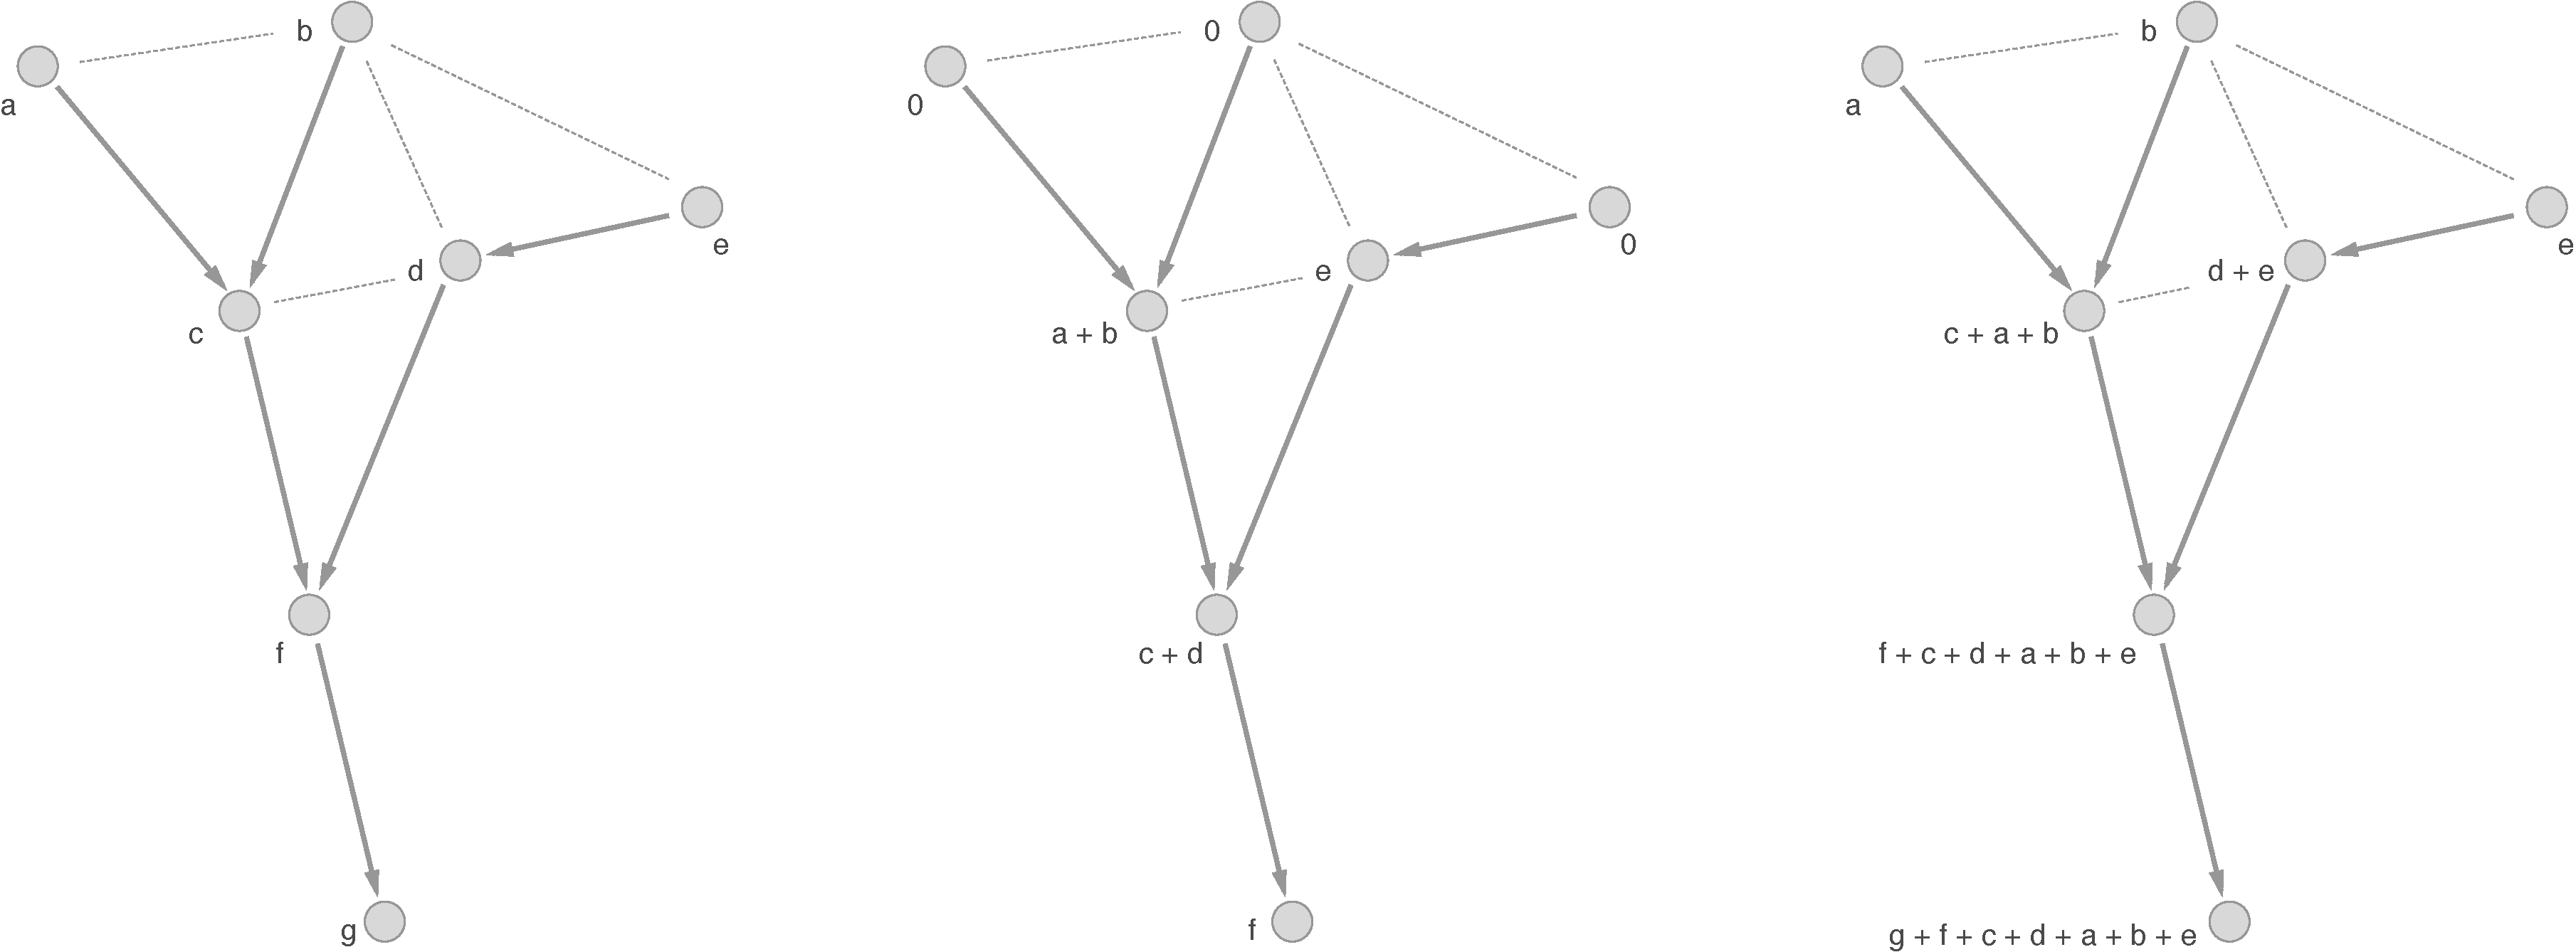
\includegraphics[width=0.9\linewidth]{FigurePDFs/Network.pdf} 
  \caption{\label{fig:Tree} The progression of information in the downhill direction for a segment of 
  a mesh representing a landscape. In (b) the information is shifted downhill (with summation). In (c), the information is accumulated at each downhill shift and produces a discrete sum of all 'upstream' information.}
\end{figure}

\section{Incremental matrix representation of downhill-flow pathways}

A directed graph such as the one illustrated in Figure \ref{fig:Tree}a can be represented by an adjacency matrix, $\bm{D}$ that represents the local connectivity of the nodes. This matrix transforms a vector of nodal values, $\bm{f}_0$ to a new vector, $f$ in which all the information has shifted to its neighbour in the direction of the arrows (which here represents the downhill direction). 
\begin{equation}
	\bm{f}_1 = \bm{D} \bm{f}_0 
\end{equation}

This operation is indicated diagrammatically in Figure \ref{fig:Tree}b with the equivalent matrix form:

\begin{equation}
\begin{bmatrix}
 0 & 0 & 0 & 0 & 0 & 0 & 0 \\
 0 & 0 & 0 & 0 & 0 & 0 & 0 \\
 1 & 1 & 0 & 0 & 0 & 0 & 0 \\
 0 & 0 & 0 & 0 & 1 & 0 & 0 \\
 0 & 0 & 0 & 0 & 0 & 0 & 0 \\
 0 & 0 & 1 & 1 & 0 & 0 & 0 \\
 0 & 0 & 0 & 0 & 0 & 1 & 0 
\end{bmatrix}
\begin{bmatrix}
 a  \\
 b  \\
 c  \\
 d  \\
 e  \\
 f  \\
 g  
\end{bmatrix} =
\begin{bmatrix}
 0  \\
 0  \\
 a+b  \\
 e  \\
 0  \\
 c+d  \\
 f  
\end{bmatrix}
\end{equation}

A second application of $\bm{D}$ moves all information another increment downhill. $\bm{D}^k$ moves information by $k$ increments in the downhill direction. Since the graph represents a flow across the landscape and has no closed cycles, all information eventually propagates to an outflow point or a local minimum in the landscape. This means that the vector $\bm{f}_N = 0$ where $N$ is the length of the longest downhill path in the network;  an equivalent statement is that $\bm{D}^N = \bm{0}$. 


\subsection{Upstream Summation}

The upstream runoff term in equation () can be computed using the adjacency matrix as follows. 

\begin{equation}
    \bm{q} = \left[ \bm{I} + 
                    \bm{D} + 
                    \bm{D}^2 + \cdots
                    \bm{D}^N + 
                    \cancel{\bm{D}^{N+1}} + \cdots +
                    \cancel{\bm{D}^{\infty}}  
                    \right] \bm{\mathcal R} 
\end{equation}
 
\begin{equation}
            \bm{q} = 
                    \sum_{i=0}^{N} \bm{D}^i \bm{\mathcal R}  \;\;\; \textrm{or} \;\;\; 
    \bm{q} = \bm{A} \bm{\mathcal R}
\end{equation}

$\bm{A}$ itself is not particularly useful as it is an unwieldy, dense matrix. To avoid the need to compute and store $\bm{A}$, we can instead compute $\bm{A} \bm{\mathcal R}$ through a recursion. We first define the partial summation of the upstream contributions after $i$ iterations as 

\begin{equation}
     \bm{q}_i = \sum_{i=0}^{i} \bm{D}^i \bm{f} 
\end{equation}

To compute $\bm{q}_(i+1)$, we observe that 

\begin{equation}
     \bm{q}_{i+1} = (\bm{I} + \bm{D}) \bm{q}_i
\end{equation}

$\bm{I}+\bm{D}$ is a very sparse matrix that can be built once and repeatedly applied to each successive $ \bm{q}_i$ in order to compute $\bm{q}$. This operation can take full advantage of purpose-built, efficient linear algebra routines including those provided by parallel libraries such as PETSc. 

We also note that the extreme sparsity of $D$ can work against computational efficiency due to a high ratio of memory access to calculation and, in parallel, a high ratio of communication to floating point operations. A simple trick to improve this ratio is to use a higher degree of recursion:

\begin{equation}
    \bm{q}_{i+2} = (    \bm{I} + 
                        \bm{D} + 
                        \bm{D}^2 )
                                \bm{q}_i
\end{equation}

or, more generally, 

\begin{equation}
    \bm{q}_{i+s} = \bm{A}_s \bm{q}_i
    \label{eq:fastrecursion}
\end{equation}  
where 
\begin{equation}
    \bm{A}_s = \sum_{j=0}^{s} \bm{D}^j 
\end{equation}
$\bm{D}^0$ is the identity matrix, and $\bm{D}^{i+1}$ is always more sparse than $\bm{D}^i$ as a result of information flowing out of the mesh. Thus the number and pattern of non-zeros of $\bm{A}_s$ can be determined relatively simply. 

Finally, the nilpotency of $\bm{D}$ means that applying the recursion (\ref{eq:fastrecursion}) does not require any special treatment when $s$ is not a factor of $N$, as additional iterations do not change the result (i.e. $\bm{q}_{N+1} = \bm{q}_{N}$ )

%% [Note this is implicitly described in Braun \& Willet]

\subsection{Multiple descent pathways}

In regions where deposition dominates and the landscape becomes increasingly flat, a single downhill direction from one point in the mesh to another is potentially a poor approximation of the actual fluid pathway and it may be more appropriate to channel flow along multiple edges in the mesh. When working with a mesh of points that is completely regular, it may also be helpful to route flow to more than one destination node in order to prevent locking of erosion pathways along the cardinal directions. [See Jean Braun for this and also see the Tucker review]

Let us define a matrix $\bm{D}_2$ to represent the adjacency relationship between a node and its second-steepest connection. The matrix that propagates information a single step in the downhill direction is now defined as
%%
\begin{equation}
    \bm{D'} =  \bm{W}_1  \bm{D}_1 + 
                  \bm{W}_2  \bm{D}_2 
\end{equation}
%%
Where $\bm{W}_{1}, \bm{W}_{2}$ are diagnonal matrices of weights that satisfy $ \bm{W}_1 +  \bm{W}_2 =  \bm{I}$ see Tucker for a typical approach to determining $\bm{W}$). The subscript $1$ is used to represent the adjacency matrix for the steepest connection, previously identified as $\bm{D}$.

The results defined above all apply if $\bm{D}$ is replaced by $\bm{D'}$. In the recursion relationship (\ref{eq:fastrecursion}), however, the story is more complicated. \begin{equation}
    \bm{A'}_s = \sum_{j=0}^{s} \left[  \bm{\bm{W}_1 D_1 + \bm{W}_2 D_2} \right]^j
\end{equation}
contains products of $\bm{D}_1$ and $\bm{D_2}$ which increases the number of computations required to build $\bm{A'}_s$. However, the structure of the matrices for products of arbitrary combinations of $\bm{D_1}$ and $\bm{D}_2$ is still that of moving information at any given point to another point and therefore the maximum number of non-zero entries in $\bm{A'}$ is predictable from the number of unique terms in the summation.

\subsection{Local minima}

The assumptions that flow from within the domain propagates to the boundary during every timestep and that there is no build-up within the domain breaks down at local minima in the landscape. Local minima should flood until they are able to re-establish a new outflow channel. It is a useful property of the $\bm{D}$ matrix that $\bm{D}^T$ propagates information to all of the uphill nodes of a given point (a one-to-many mapping in general). 
	
\end{document}


